%%%%%%%%%%%%%%%%%%%%%%%%%%%%%%%%%%%%%%%%%%%%%%%%%%%%%%%%%%%%%%%%%%%%%%
% Lớp 12 | Các số đặc trưng ... ghép nhóm | Phương sai, độ lệch chuẩn của mẫu số liệu ghép nhóm
% Dạng 2D3?2-1: Công thức lý thuyết
% Số câu: 4  (sinh tự động bởi tach_cau.py; từ nay thầy sửa trực tiếp file này)
%%%%%%%%%%%%%%%%%%%%%%%%%%%%%%%%%%%%%%%%%%%%%%%%%%%%%%%%%%%%%%%%%%%%%%

%%%%%%%%%%%%%%%% TRẮC NGHIỆM 4 PHƯƠNG ÁN %%%%%%%%%%%%%%%%

% nguồn: Lop_12_Dai_so_Chuong_3
\begin{ex}%[2D3T2-1]%[ma:166f88f5]
	\immini{ 
	Một vật chuyển động trong  $3$ giờ đầu với vận tốc $v$ km/h phụ thuộc thời gian $t$ (h) có đồ thị là một phần của đường parabol có đỉnh $I(2;9)$ và trục đối xứng song song với trục tung như \textit{Hình 4.30}. Tính quãng đường $s$ mà vật di chuyển được trong $3$ giờ đó.
	 \choice
		 {$s=25,25$ km}
		{$s=24,25$  km}
		{\True  $s=24,75$ km}
		{$s=26,75$ km} 
		} 
		 {\hspace{0.5cm}
		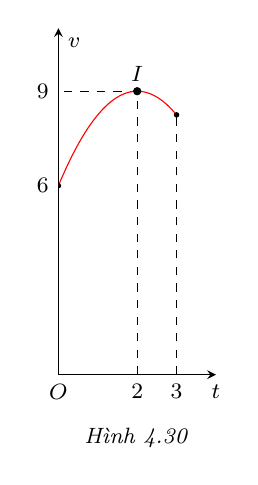
\begin{tikzpicture}[scale=0.5,>=stealth,x=1cm,y=0.8cm]
				\draw[->] (0,0)  -- (4,0) node [below] {\footnotesize $t$};
				\draw[->] (0,0) --  (0,11) node [below right] {\footnotesize $v$};
				 \draw (0,0) node[below] {\footnotesize $O$};
				\draw[dashed,thin](2,0) node[below] 
					{\footnotesize $2$}--(2,9) node[above]{\footnotesize  $I$}--(0,9) node[left]{\footnotesize $ 9$}
					(3,0)  node[below]{\footnotesize $3$}--(3,8.25)
					(0,6) node[left]{\footnotesize $6$}; 
				\draw (2,-2) node {\footnotesize  \textit{Hình 4.30}};
				\clip (0,0) rectangle  (4,10);
				\draw[smooth,red,samples=100,domain=0:3] plot (\x,{(-3/4)*(\x)^2+3*(\x)+6}); 
				\fill (0,6) circle[radius=2pt] (3,8.25) circle[radius=2pt] (2,9)  circle[radius=3pt];
			\end{tikzpicture}
		\hspace{0.5cm}} 
	\loigiai{ 
		Theo đề bài, đồ thị là một phần của đường parabol có đỉnh  $I(2;9)$ và đi qua điểm $M(0,6)$.\\
		Gọi  $v(t)=a(t-2)^2+c$.\\
		Ta có $\heva{ 
		&  I(2;9) \in (P)\\
		& M(0,6) \in (P) 
		 }
		\Leftrightarrow  \heva{
		&  c=9\\
		 & 6=a\cdot(-2)^2+9}
		\Leftrightarrow \heva{ 
		& c=9\\ 
		& a=-\dfrac{3}{4}.} 
		$\\ 
		Suy  ra $v(t)=-\dfrac{3}{4}\left(t-2\right)^2+9$.\\
		Vậy quãng đường đi được trong $3$ giờ  đó là $s=\displaystyle\int_0^3v(t)\mathrm{\,d}t=24,75$ km.
	} 
\end{ex}

% nguồn: Lop_12_Dai_so_Chuong_3
\begin{ex}%[2D3Y2-1]%[ma:c21fefce]
	 Tích phân $ \displaystyle\int_0^1
	(e^x-4x^3)\mathrm{\,d}x $ bằng 
	\choice 
		{\True $ e-2  $}
		{$ e-1  $}
		{$ e-4  $}
		 {$ e-3 $}
	\loigiai{ 
		$ \displaystyle\int_0^1 
		 \left(e^x-4x^3\right)\mathrm{\,d}x=\left(e^x-x^4\right)|_0^1=\left(e^1-1\right)-\left(e^0-0\right)=e-2 $.
	} 
\end{ex}


%%%%%%%%%%%%%%%% TRẢ LỜI NGẮN %%%%%%%%%%%%%%%%

% nguồn: Lop_12_Dai_so_Chuong_3
\begin{bt}%[2D3B2-1]%[ma:a7fcebe9]
	Cho $\displaystyle \int_{-1}^{3} f(x)\mathrm{\,d}x  = 7$. Tính $\displaystyle \int_{-1}^{3} [f(x)+4x]\mathrm{\,d}x$.
	 \shortans{23}
	\loigiai{ 
		Ta có $\displaystyle \int_{-1}^{3} [f(x)+4x]\mathrm{\,d}x = \displaystyle \int_{-1}^{3} [f(x)]\mathrm{\,d}x + \displaystyle  4\int_{-1}^{3} x\mathrm{\,d}x = 7 + 16 =23 $.
	} 
\end{bt}


%%%%%%%%%%%%%%%% TỰ LUẬN %%%%%%%%%%%%%%%%

% nguồn: Lop_12_Dai_so_Chuong_3
\begin{bt}%[2D3T2-1]%[2D4V3-2]%[ma:f4a398e8]
	\immini{Mặt cắt ngang của một ống dẫn khí nóng là hình vành khuyên như hình vẽ. Khí bên trong ống được duy trì ở $150^{\circ} C$. Biết rằng nhiệt độ $T\left(^{\circ} C\right)$ tại điểm $A$ trên thành ống là hàm số của  khoảng cách $x~(\mathrm{cm})$ từ $A$ đến tâm của mặt cắt và
	$$ 
	T^{\prime}(x)=-\dfrac{30}{x} \quad(6 \leq x \leq  8).
	$$ 
	Tìm nhiệt độ mặt ngoài của ống.}{\begin{tikzpicture}[scale=1,font=\footnotesize,line join=round,line cap=round,>=stealth,line width=1pt]
		\coordinate (O)  at (0,0);
		\draw[fill=yellow,name path=C1] (O)  circle (3 cm);
		 \draw[name path=C2] (O) circle (2 cm);
		\draw[name path=C3,dashed] (O) circle (2.7 cm); 
		\draw[fill=white,name path=C1] (O) circle (2.4 cm); 
		 \coordinate (A) at ($(O) + (40:2.7)$);
		\coordinate (B) at ($(O) +  (110:2.4)$);
		\coordinate (C) at ($(O)  + (190:3)$);
		\draw (O)--(A) node[midway,above left,font=\small]  {$x$ cm};
		\draw  (O)--(B) node[midway,above left,font=\small] {$6$ cm};
		\draw  (O)--(C) node[midway,below right,font=\small] {$8$ cm};
	\end{tikzpicture}
	} 
	\loigiai{Ta có $T(6)=150$ (khí bên trong ống được duy trì  ở $150^{\circ} C$).
		 $$
		\begin{aligned}
			T(8)-T(6)  &=\displaystyle\int_6^{8} T^{\prime}(x) \mathrm{\,d}x=\displaystyle\int_6^{8}-\dfrac{30}{x} \mathrm{\,d} x \\
			&=-30 \displaystyle\int_6^{8}\dfrac{1}{x} \mathrm{\,d}  x \\
			&=\left.-30\ln  x\right|_6 ^{8}\approx -8{,}63.
		\end{aligned}
		 $$
		Suy ra $T(8)=T(6)-8{,}63\approx 141{,}37$ ($^{\circ}  C$).\\
	Vậy nhiệt độ mặt ngoài của ống là $141{,}37^{\circ} C$.} 
\end{bt}
